% Author: Jørn Olav Jensen

\newpage
\section{Suggested solutions: Arbitrary Frequency Response Filters}
\begin{enumerate}
    % Exercise 1
    \item Consider two signals of the form:
          \begin{align*}
              x_{1}[n] & =\sum_{i=1}^{5}A_{i}\cos(2\pi f_{i}i) + w_{n},              \\
              x_{2}[n] & =a_1\delta[n-8192] + a_2\delta[n-9192] + a_3\delta[n-7192],
          \end{align*}
          where $|A_{i}|>|a_{j}|$ for every pair $i, j$, here $w_n$ is white noise.
          \footnote{White noise is considered as a random variable with a normal distribution
              with $\mu=0$ and variance $\sigma^{2}=1$ here} In Listing \ref{code17_1} is code to generate these signals and plot them.

          \lstinputlisting[language=Python, caption=Example signal code, label=code17_1, linerange={0-27}]{ch17/code/ex17_1.py}

          \begin{marginfigure}
              \centering
              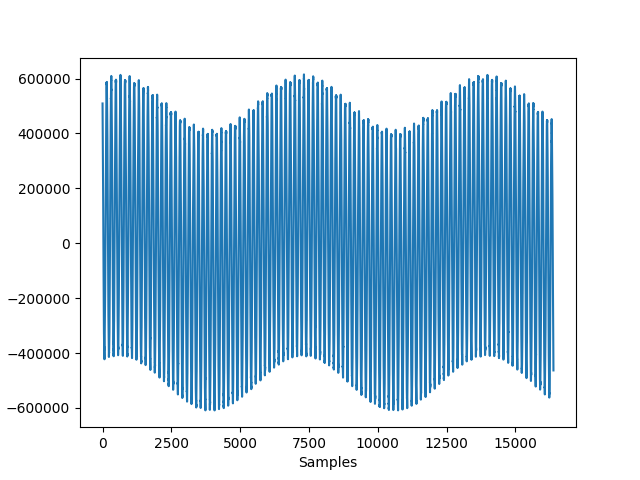
\includegraphics[width=7.5cm, height=7.2cm]{ch17/figures/ex17_1.png}
              \caption{Noisy signal we want to filter}
              \label{fig17_1}
          \end{marginfigure}

          \begin{enumerate}[a)]
              % Exercise 1a)
              \item To estimate the spectrum, we use the Hann window to avoid spectral leakage.
                    The code for computing the spectrum using the Hann window is shown in Listing \ref{code17_2}.

                    \lstinputlisting[language=Python, caption=Spectrum for noisy signal in Figure \ref{fig17_1}, label=code17_2, linerange={0-40}]{ch17/code/ex17_1a.py}

                    \begin{marginfigure}
                        \centering
                        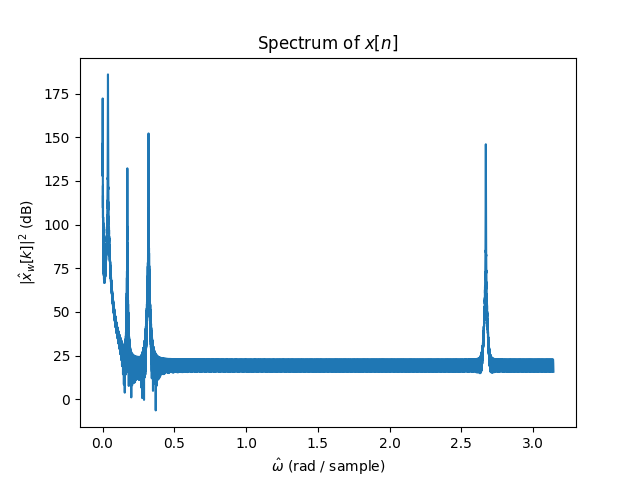
\includegraphics[width=7.5cm, height=8.0cm]{ch17/figures/ex17_1a.png}
                        \caption{Spectrum in dB for the signal shown in Figure \ref{fig17_1}}
                        \label{fig17_2}
                    \end{marginfigure}

                    % Exercise 1b)
              \item To filter out the noise, we use a filter that will remove strong spectral components and keep the
                    weak components constant at $1.0$. That is, our filter will be:
                    \[\hat{h}[k]=\begin{cases}
                            \frac{1}{|\hat{x}_{w}[k]|}, \quad \text{for strong spectral components}, \\
                            1, \quad\quad \text{otherwise}.
                        \end{cases}\]
                    Where $\hat{x}_{w}[k]$ is the Hann windowed tapered signal. Looking at the spectral power, we can determine which components need to be lowered.
                    After doing this we apply the inverse DFT to obtain our filtered signal,
                    \[ x[k]=\mathcal{F}_{D}^{-1}\{\hat{x}_{w}[k]\hat{h}[k]\}. \]
                    The implementation of this is shown in Listing \ref{code17_3}.

                    \lstinputlisting[language=Python, caption=Filtering of the signal, label=code17_3, linerange={0-60}]{ch17/code/ex17_1b.py}

                    Running this code will generate the plots shown in Figure \ref{spectral_pw17} and \ref{filtered_signal}.

                    \begin{marginfigure}
                        \centering
                        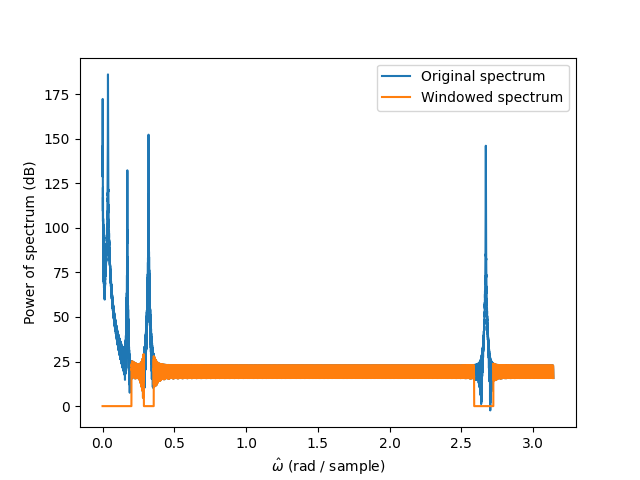
\includegraphics[width=7.5cm, height=7.0cm]{ch17/figures/spectral_pw.png}
                        \caption{The comparison of the spectral power}
                        \label{spectral_pw17}
                    \end{marginfigure}

                    \begin{figure}
                        \centering
                        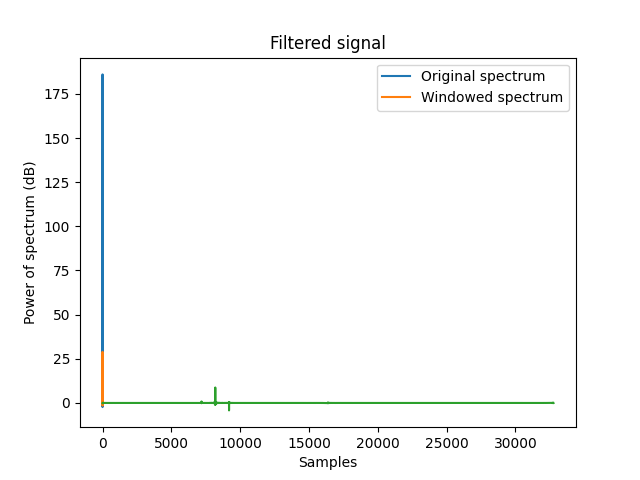
\includegraphics[height=9.0cm]{ch17/figures/filtered_signal.png}
                        \caption{Filtered signal, the weak signal is now visible}
                        \label{filtered_signal}
                    \end{figure}

                    % Exercise 1c)
              \item The filter in this case reduces the strong frequencies while at the same time keeping lower frequencies fixed.
                    The effect is that the original signal which had a lot of noise coming from $x_{1}[n]$ will have that
                    noise significantly reduced. The remaining information in the signal is the other part, being $x_{2}[n]$,
                    which consists of unit impulses for which the frequency components were kept at $1$.
                    Therefore, the filtered signal looks like $x_{2}[n]$ even though a lot of frequency components have been removed.
          \end{enumerate}


\end{enumerate}